\documentclass{sigchi}

\pagenumbering{arabic}% Arabic page numbers for submission. 

% Use \toappear{...} to override the default ACM copyright statement (e.g. for preprints).

% Load basic packages
\usepackage{balance}  % to better equalize the last page
\usepackage{graphics} % for EPS, load graphicx instead
 \usepackage{times}   %comment if you want LaTeX's default font
\usepackage{url}      % llt: nicely formatted URLs

% llt: Define a global style for URLs, rather that the default one
\makeatletter
\def\url@leostyle{%
  \@ifundefined{selectfont}{\def\UrlFont{\sf}}{\def\UrlFont{\small\bf\ttfamily}}}
\makeatother
\urlstyle{leo}


\usepackage{etoolbox}
\makeatletter
\patchcmd{\maketitle}{\@copyrightspace}{}{}{}
\makeatother


% To make various LaTeX processors do the right thing with page size.
\def\pprw{8.5in}
\def\pprh{11in}
\special{papersize=\pprw,\pprh}
\setlength{\paperwidth}{\pprw}
\setlength{\paperheight}{\pprh}
\setlength{\pdfpagewidth}{\pprw}
\setlength{\pdfpageheight}{\pprh}

% Make sure hyperref comes last of your loaded packages, 
% to give it a fighting chance of not being over-written, 
% since its job is to redefine many LaTeX commands.
\usepackage[pdftex]{hyperref}
\hypersetup{
pdftitle={Revisiting User Confidence in Smartphone Privacy and Security Vigneswaren, Roshandel},
pdfauthor={Vigneswaren, Roshandel},
pdfkeywords={mobile phone usage, user confidence, application installation, smartphones},
bookmarksnumbered,
pdfstartview={FitH},
colorlinks,
citecolor=black,
filecolor=black,
linkcolor=black,
urlcolor=black,
breaklinks=true,
}

% create a shortcut to typeset table headings
\newcommand\tabhead[1]{\small\textbf{#1}}


% End of preamble. Here it comes the document.
\begin{document}

\title{Revisiting User Confidence in Smartphone Privacy and Security}

% Note that submissions are blind, so author information should be omitted
\numberofauthors{2}
\author{
  \alignauthor Kapil Haresh Vigneswaren\\
    \affaddr{Cheriton School of Computer Science}\\
    \affaddr{University of Waterloo}\\
    \affaddr{Waterloo, ON, Canada, N2L 3G1}\\
    \email{khvignes@uwaterloo.ca}\\
  \alignauthor Hirad Roshandel\\
    \affaddr{Cheriton School of Computer Science}\\
    \affaddr{University of Waterloo}\\
    \affaddr{Waterloo, ON, Canada, N2L 3G1}\\
    \email{hroshand@uwaterloo.ca}\\
}

% Teaser figure can go here
%\teaser{
%  \centering
%  \includegraphics{Figure1}
%  \caption{Teaser Image}
%  \label{fig:teaser}
%}

\maketitle

\begin{abstract}
In 2012, a study by Chin et al. revealed that smartphone users do not feel confident at performing certain tasks such as accessing financial information, health data, entering social security number and providing other personal information on their smartphones. Participants in Chin's study were mainly concerned about losing their smartphones, physical damage, data loss and (lack of) backup, and trusting applications. Both Apple and Google have introduced new technologies such as fingerprint and face detection for authentication, and Apple Pay and Android Pay for contactless payments. In this study we re-evaluate user confidence in smartphone privacy and security, and investigate whether recommendations put forward by Chin et al. have been applied in real life. We conducted a user study with 33 respondents, where we got users to complete a survey that allowed us to learn more about how our users used their devices, the factors they take into account when getting apps, the confidence that their privacy and security is maintained when they are doing various activities on their smartphone, what other concerns they had with regards to their smartphone, and if they felt the solutions provided in the original paper were implemented and effective in improving user confidence in smartphone privacy and security. We then compared our data with the data presented in the original paper to identify the differences (improvements or otherwise), as well as similar trends in the data. Our findings allow us to present a more up to date picture of the current landscape of smartphone privacy and security from the user's point of view.  
\end{abstract}

\keywords{
	Mobile phone usage, Mobile security, Application installation, Smartphones}
    
\section{1. Introduction}
Over the last few years smartphone ownership rates have been skyrocketed in many emerging economies due to variety of devices and relatively affordable prices. A recent study conducted from March 25 to May 27, 2015 has shown that the highest rates of smartphone ownership are among the richer economies. This includes 88\% of South Koreans, 77\% of Australians, 74\% of Israelis and 72\% of Americans \cite{poushter}. This number is significantly higher than the previous result in 2011 showing smartphone penetration of 35\% in United States. In 2011, mobile online shopping was only 3\% of overall shopping revenues \cite{chin2012measuring}, indicating that users were hesitant to perform these tasks on their smartphones. However, by the end of 2016, it is expected that smartphone users spend \$31 billion shopping using their phones \cite{IanBlair}. New technologies such as Apple Pay, Android Pay, and mobile digital assistant technologies, such as Google Now, Siri and Cortana have been introduced to facilitate and assist smartphone users with tasks which  previously users were hesitant to perform. This drastic change could indicate that users' confidence level in smartphone security and privacy may have been improved over the past few years.

In a 2012 user study \cite{chin2012measuring}, Chin et al. argues that users are more apprehensive about performing privacy sensitive (Social Security Number, Health data, etc.) and financial tasks such as accessing bank account and making a purchase on their smartphones in comparison to their laptops. Other studies also have shown that users often begin tasks on smartphones but complete them on their computers \cite{bao2011smart} \cite{karlson2009working} \cite{matthews2009no}. Chin argues that these platform switches are due to screen size, network performance, typing difficulties or  security concerns. The main results of their user study indicate that users are more willing to experiment with applications on their mobile phones compared to their laptops. They are more likely to install free, non-brand-name applications on their mobile phones, and they often discover them via browsing or advertisements. From the privacy and security aspect, participants also do not greatly consider existing security indicators like privacy policies, end user license agreements (EULAs) and sensor permissions. Instead, they rely on user reviews and popularity to evaluate the quality and safety of applications. Chin speculates that these installation habits can potentially put users in a higher-risk situation comparing to laptop installation habits. Participants in Chin's study were mainly concerned about physical damage, physical phone loss and theft, data loss and back up, battery life, reception strength and signal, and trusting applications on their smartphones. Chin's paper provides few recommendations in order to improve overall smartphone security and allow users to confidently understand the full potential of their mobile applications. Some of these recommendations include educating users about the security properties of the different media and the benefits of end-to-end encryption, new security indicators to help smartphone users identify trustworthy brands, improved user interfaces for sensitive applications, better backup solutions, and better remote locking and remote wiping services. 

In this paper we are trying to investigate whether these sentiments have changed over time, now that more people have embraced the smartphone technology. New technologies for mobile payments such as Apple Pay and Android Pay, biometric based authentication system using fingerprint scanners and facial recognition technologies, and device tracking technologies have been introduced over the last few years which we believe could have an effect on users feeling more comfortable and confident in using their smartphones in comparison to Chin's 2012 user study. Our main goal by the end of this study is to see if the concerns raised by Chen et al.'s paper have been addressed and whether the recommendations put forward by them have been applied in reality. We would also want to provide a more up to date picture of the current landscape of user confidence in terms of the security and privacy of smartphone.

\textbf{Contributions.} This paper makes the following contributions:
\begin{itemize}
  \item We evaluate whether users are more willing to perform privacy sensitive tasks such as online shopping, accessing financial information, health data, etc. on their smartphones. We then compare our findings with the results found by Chin et al. in 2012.
  \item We investigate whether the proposed recommendations by Chin et al. have been implemented in current smartphones and evaluate their effectiveness in increasing security and privacy.
\item We provide a more up-to-date picture of the current landscape of user confidence in the security and privacy of smartphones.
\end{itemize}

\textbf{Hypothesis.} We hypothesize that users today take advantage of new mobile payment systems (Android Pay and Apple Pay) as well as biometric based authentication systems and feel confident that their privacy and security is preserved when using these systems. We also hypothesize that users are now less concerned about losing their devices due to the advent of automated backup services and lost device tracking services, and are more confident about their privacy and security in general on their smartphones compared to the original study by Chin et al.
\section{2. Background Knowledge}
\subsection{Android}
Google Play is still the biggest marketplace for Android users to download applications. In 2014, Google reported \cite{googlereport} that under 1\% of Android devices had potentially harmful apps installed. Google uses a server-side malware scanner to protect end users by preventing the installation and usage of malicious Android apps. However, some researchers have been able to by pass this security measure and upload malicious applications to the store \cite{googleshort}. In 2015, Google announced \cite{kim2015creating} a new review process where apps submitted for approval are manually reviewed by a team of employees at Google before the software is published on the Play Store to improve experience for both developers and users. Despite all the effort, numerous malicious applications have recently been found on the market \cite{goodin}. Thus, installing anti-virus and security applications is recommended. Google  introduced their fingerprint API and Android Pay to enhance user authentication and contactless payments respectively. In this work we investigate whether these technologies have been adopted by smartphone users.
\subsection{iOS}
The App Store is still the only official marketplace for downloading iOS applications. Apple still manually processes every application submission to ensure it is following their guidelines. Although Apple follows a more strict review process than Google, hundreds of apps on Apple's  App Store were found to be stealing personally identifiable information in 2015 \cite{brown}. In 2016, Apple mandated all applications to support ATS security protocol by 2017 which is transferring all app data over HTTPS connections instead of HTTP to reduce the potential of user exposure to nefarious code or data theft \cite{ats}. Similar to Android, iOS also supports fingerprint scanning for authentication and Apple Pay for contactless payments. We will investigate the degree of their adoption by users in this work.

\section{3. Related works}
There has been several studies conducted which all have been released about the same time or after the original paper by Chen et al. In this section we briefly discuss some of these works:

Felt et al. \cite{felt2012ve}, and King \cite{king2012come} explore the privacy and security concerns of smartphone users, and privacy and security expectations of smartphone users respectively. However, since both of these papers were published in 2012 and the newer technology could not been investigated in their work, their results have become relatively of date. 

Egelman et al.'s paper \cite{egelman2014you} examines why users choose to employ locking mechanisms and their perceptions and awareness about the sensitivity of the data stored on their devices. Although they observe a strong correlation between use of security features and risk perceptions, they only focus on the motivation to lock a device and do not evaluate any other security measure that can affect user perception about smartphone security. 

Benenson et al.'s 2013 paper \cite{benenson2013android} investigates the differences in attitudes and behavior between Android and iOS users concerning security and privacy when using applications. However, their study lacks detail and coverage, and they claim that their results are ambiguous. We aren't aware of any other paper that has followed up with the findings in the original Chen et al. paper.

\section{4. Methodology}
For our study, we decided to perform a user survey where we asked our participants to complete on their laptops. This user survey was hosted on \textit{Google Forms}. Due to our limited time, our goal was to find 25 - 30 participants. We believe this is a reasonable number since the original paper had 60 participants over the period of two months, while we are trying to achieve half of this number in the period of 2.5 - 3 weeks. We were successfully able to collect a total of 33 responses, from November 19 2016 till December 6 2016.

Prior to commencing our study, we had obtained ORE approval to conduct our user survey. Participants were also compensated \$10 for their time. Participants signed the consent forms before they participated in the survey, and at any point in time of the study, were allowed to end their participation in the user survey without affecting their compensation.
\subsection{4.1 Study Structure}
The study was designed in a way that we incorporated some of the questions from the original study by Chin et al., with some new questions. One thing to note is that we have shifted our focus to smartphone usage patterns  in our study, whereas the original paper also studied the usage patters and user confidence on desktop and laptop computers. The reason for this shift is because we already have a good baseline on the confidence level of users when working with computers, and in the last 4 years (the original paper was published in 2012), we did not see as much of a shift in the desktop computing environment compared to the smartphone environment. A copy of the survey is present in the appendix section of this paper.

\subsection{4.2 Recruitment}

We decided to advertise the study by word of mouth. We tried to avoid recruiting people who have prior knowledge of working on smartphone privacy and security, which led to some amount of screening on our users. We only recruited participants who currently use an Android or iOS smartphone. These were the challenges we faced, as we tried our best to reach our target number of participants within the limited time available.

\subsection{4.3 Limitations}

There were some limitations in terms of recruitment of participants and our methodology of the survey. First, there was a gender and age bias present in our respondents, where around 67\% of our respondents identified as male, and about 88\% of our respondents were between the ages of 18 - 34, with nearly 61\% of our respondents being between the ages of 18 - 24. This bias was unavoidable to some extent, due to the study being conducted at the University of Waterloo. About half of our respondents had occupations in the computer or mathematical fields, which is also due to the limitation of the university generally having more students and staff in this field. However, we argue that despite people being in this field, not many of them are in the security and privacy field, since we have limited that number during our screening when we advertised the study by word of mouth. The time limitation in obtaining a large enough sample to cancel out the biases also was an issue, which would be an avenue for future work.

\section{5. Results}

\subsection{5.1 Demographics}

As mentioned in the previous section, we had 66.7\% of our respondents (22 respondents) who identified as male, while 30.3\% of them (10 respondents) identified themselves as female, and 3.1\% (1 respondent)  preferred not to disclose their gender. Our participants were primarily aged between 18 - 24 years, with 60.6\% of them falling in this group. The next largest age group was the 25-34 years old age group with 27.3\% respondents and finally 3\% and 9.1\% of our participants in the 35-44 years old age group and 45-54 years old age group respectively.

Considering that our study was conducted in a university town, with a university popular for computing and mathematics programs, it was unsurprising to see that 51.5\% of our participants worked in this field. The next largest occupation field was the "Other occupations" which upon further checks indicated that these were respondents who claimed that they were students, but did not disclose what field they were in. We also had a number of respondents from the education sector as well as the architecture and engineering sector , and 1 respondent in the business sector and 1 in the installation, maintenance and repair sector.

\subsection{5.2 Smartphone Usage}

Most of our participants had been using iOS and Android smartphones in the past, which is consistent to prior statistics indicating that these two operating systems have been the top two operating systems since Q4, 2011 \cite{statista_2016}. While statistics indicate that Android has a greater market share than iOS, our survey data suggested otherwise, but this could be due to the location where our survey was conducted, as it is known for Android to be popular in developing markets. It was also noted that we had nearly double the number of iOS users compared to Android users. For the most part, we could say that our participants were reasonably well versed with the way a smartphone operates, as over half of them had been using one for more than 5 years. Only 4 participants, which was 12.1\% of our participants had between 1 - 3 years of experience with smartphones, which was the least amount of experience in using a smartphone among our participants.

Nearly all of our participants, except 1 participant did not share their smartphone with someone else on a regular basis, and the one person who shared their smartphone mentioned that they shared it with family members. Our user group did not seem too conservative in terms of trying out apps from unknown brands or companies, with a staggering 82\% of them stating that they would be at least somewhat likely to try out such apps. In terms of the type of apps that people tend download, most participants responded that they would install social apps, followed by utilities, games and productivity apps on their device. We noticed a decent number of people responding that they would have educational apps installed on their device too, which is not surprising due to the location of the survey. However, only 3 respondents (2 on Android and 1 on iOS) mentioned that they would install security apps on their device. All of our users mentioned that they search for their applications from their respective app stores, with a few also depending on Google searches as well.

A decent number of our participants have auto update turned on for their smartphone operating system, or apply updates immediately when they are made available, and with less than 10\% never updating the OS of their smartphone. Also, as expected considering our target demographic, most of our users have indicated that they are able to install applications on their own without assistance from others.

Moving on to backup and security trends, our data suggests some interesting trends. Near two-thirds of our participants did not use lost phone tracking services and less than half of them used automatic backup services. There was an equal distribution between Android and iOS users who did not use automatic backup services. However, on the virus protection front, just 1 Android user had an anti-virus application installed.

\subsection{5.3 Anti-virus Purchase \& Usage Habits}

The lone participant who had an anti-virus application installed on their smartphone indicated that it was a free application, by AVG. The participant had heard about the application from a family/friend and had obtained the application via Google Play Store. Despite first hearing about the application from a family/friend, the participant considered the search ranking of the application, other user reviews, the ease of installation and the familiarity of the brand, before installing the application. They also noted that they used the application on a weekly basis.

Despite 3 users saying that they tend to install a security application, only 1 participant had it installed at the time of our survey. Having just 1 respondent's data does not really allow us to identify patterns or significant findings in terms of the purchase and usage habits of anti-virus applications among smartphone users.

\subsection{5.4 Non-Security Application Purchase \& Usage Habits}

In this section, we focus on non-security related applications that are installed on the participant's device.
\begin{figure}[h]
    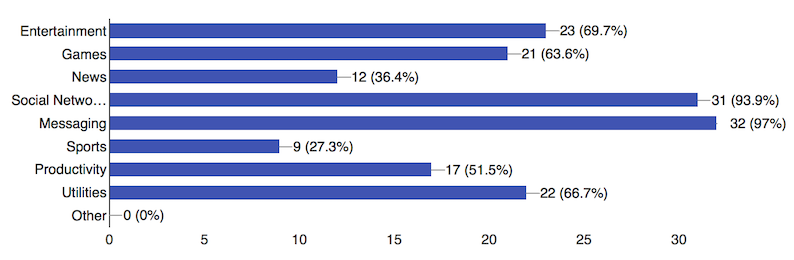
\includegraphics[height=3cm]{categories}
    \caption{Categories of applications installed on participants' smartphones}
    \label{fig:applicationtypes}
\end{figure}

We noted that everyone except 1 participant had some form of a messaging app installed, and 31 out of 33 of them had social network apps installed - which seems consistent to the earlier question that gauged the tendency for our participants to install an application. Entertainment apps came in next, with 23 of our respondents having such apps installed on their device, closely followed by the utilities category and games category. Only slightly over half of our users had productivity apps installed, which again was close to the numbers we saw in the question on their installation tendencies. There were about a third of our respondents who mentioned that they had news apps installed and just under 30\% had sports applications installed on their device.

Despite over 50\% of respondents being from the computing or mathematics field, which would indicate that they were likely to know the ways of installing third party applications via other means like sideloading (especially on Android), it was unexpected that all respondents got their applications from the respective app stores for their smartphones, as we expected at least one or two respondents to have used other methods to install applications.

Most of our respondents mentioned that they had heard about the apps they had for the first time from their friends and family or via the featured sections of their respective app stores. They also heard about apps from non family members/friends, as well as from browsing the Internet or in articles. Slightly less than a third heard about apps through advertisements, and only 10\% of our respondents said that they were forced into installing an application - which is an indication that our user base seemed to have control over the apps that were installed on their smartphones.

Price, popularity of the application and user reviews, in that particular order were the top three criteria users generally considered before installing the applications, followed by friends and family recommendation as well as screenshots. Interestingly, expert reviews and recommendations from physical stores were not held in high regard, and we had one user who mentioned, that they also considered the usefulness of an application prior to installing it. Although it was encouraging to see that a third of our users generally considered the permissions the apps requested, only 5 people considered the application's privacy policy and just 1 person considered the end user license agreement installing an application. We expected a larger number of people to have considered the privacy policy and the license agreement, considering that about half of our respondents were from the computer or mathematics field.

\subsection{5.5 Installation Factors}

In this section, our goal was to delve much deeper the importance of a number of factors users may consider when installing an application. For each of the criteria, our respondents were given the following options: \textit{ Always consider, Sometimes consider, Rarely consider, and Never consider}.

\begin{figure}[h]
    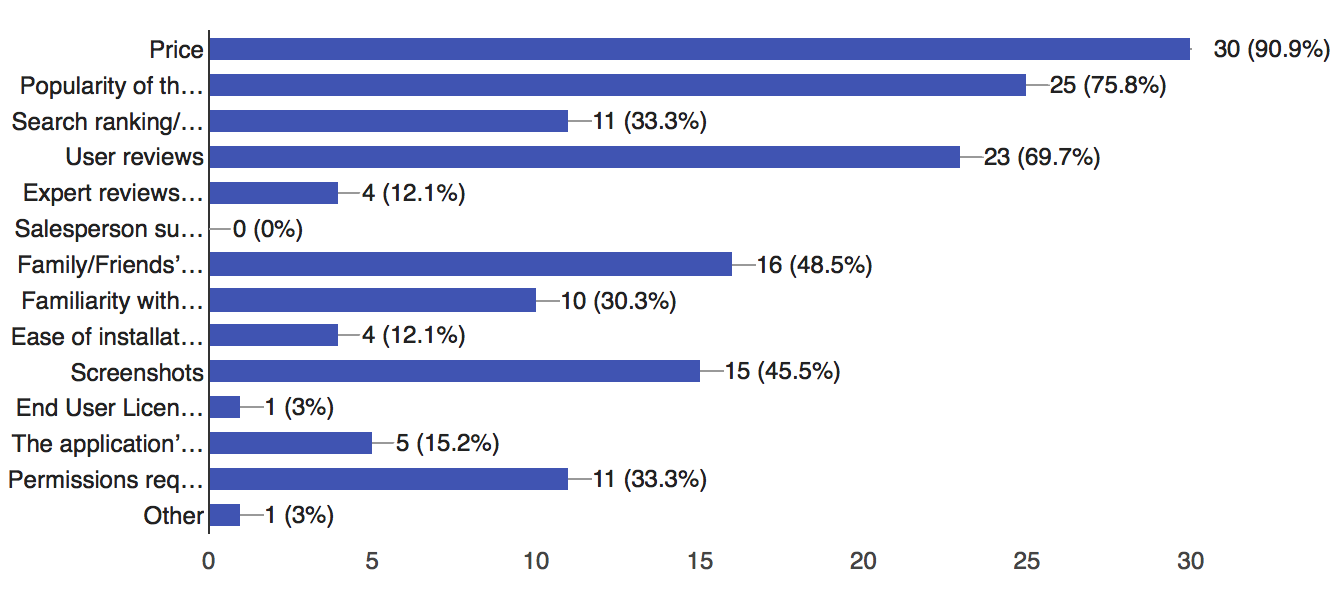
\includegraphics[height=4.2cm]{factors}
    \caption{Factors considered by users prior to installation}
    \label{fig:installFactors}
\end{figure}

Price had to be one that had a clear distinction, where a staggering 84.8\% of our respondents indicated that they always considered the price of the application before installation. Only 3 respondents, which makes up about 9\% of our respondents, had responded that they rarely or did not consider the price of the application, which is not surprising considering people are less likely to spend on apps that they may find  useful. Slightly over half of our respondents had sometimes considered the popularity of an application before they installing it, while near 40\% always considered the popularity of an application - in fact, just 2 participants did not fall in either of these two options. These two respondents indicated that they never considered this criteria. 

The majority of our respondents (39.4\%) indicated that they sometimes consider search ranking or sponsored listings, with 30.3\% saying that they rarely considered this criteria. Only 15.2\% said that they always considered this criteria. This seems reasonable based on the factors that our users generally considered. The majority of our users also had sometimes considered the user reviews of a particular application, but this time, unlike the sponsored listings, there were more people who had always considered this criteria. In this case, all but 9.1\% of our respondents indicated they at least sometimes or always considered the user reviews.

The strong preference for user reviews however does not translate the same way for the expert reviews. In this case, 68.7\% of our users either rarely or did not consider these expert reviews, with the majority of our users ( 40.6\% of our respondents) mentioning they sometimes considered this criteria.Only 1 respondent said that they always considered expert reviews. This divide between user and expert reviews seems consistent to results from the earlier question on which factors our respondents generally considered before installation. The similar trend also applies to the suggestions from the salesperson at a physical store, where 94\% of our respondents rarely or did not consider such recommendations. Delving deeper, it was clear that people never considered such recommendations, judging by the significant 78.8\% of our respondents who chose this option, and not even one person saying that they always considered these recommendations.

There was a relatively strong preference for recommendations from family and friends, where 81.3\% of our respondents indicated that they sometimes or always considered such recommendations, with a slightly larger proportion of them stating that they had sometimes considered over the always considered option. Brand familiarity too was another criteria that our users seemed to consider to some extent, but not very strongly. Nearly 70\% of our respondents indicating that they either sometimes, or always considered this, though there were more who had sometimes considered this, over those who always considered it. Ease of installation was a criteria that many of our users also considered, with nearly two-thirds of them stating that they would sometimes or always consider this criteria - in this case, the number who always considered ease of installation was near equal to the number of those who sometimes considered this criteria. It was interesting to see an equal number of people who rarely considered ease of installation, as well as the number of those who did not consider this.

Screenshots was the surprising result in this case as we did not expect that many people to consider it, but it seemed that 72.7\% of our users had sometimes or always considered screenshots before installing an app, with 42.4\% of our users always considering this criteria. This could be due to the fact that screenshots give users an idea on how the app would function in real life, before they had installed it - allowing them to judge, to some extent before they get the app. 

The disappointing result had to be the lack of awareness on the end user license agreement (EULA) and the privacy policy of the application. As initially indicated by the lack of people who even generally considered this when they got apps, only a mere 18.2\% of our respondents had sometimes or always considered the EULA of an app. In fact, just 3\% of our respondents (1 respondent) always considered it, while 63.6\% never considered this. This divide in responses was not as large in the case of the privacy policy, however. While only 30.2\% of our respondents had either sometimes or always considered this, 12.1\% of our respondents had always considered the privacy policy. In fact, the number of people who did not consider the privacy policy was significantly less, with 42.4\% of users never considering the privacy policy (significantly less than the EULA). In the case of permissions, we noticed a better result, slightly more than half of our users had considered the permissions requested by an app sometimes, or always. We noted a slightly larger proportion of users who always considered the permissions requested (at 30.3\% of respondents), over those who only considered this sometimes. We had an equal number of respondents (24.2\% each) who never considered the permissions requested or rarely considered this criteria. These numbers were encouraging, but still could be improved on.

\subsection{5.6 Confidence When Using a Particular Feature on a Smartphone}
The goal of this section was, given some activities that are likely to be conducted by people on their devices, we wanted to find out how confident users were that their security and privacy was maintained when conducting such activities. This data would be very useful in the sense that it allows us to identify weaknesses in existing implementations, to allow us to make users feel more confident that their privacy and security is being preserved when using such features - as having this confidence would make more users use such features. Respondents gave a rating of 0-5, which denoted, 0 - never used this service, 1 - very unconfident, 2 - unconfident, 3 - average/neutral confidence, 4 - confident, 5 - very confident.

We began with asking our respondents about their confidence in using navigation applications on their smartphones that use their location. In this case, all but 1 respondent had used this service, and there was a clear sign that the majority of our respondents were confident of this service, with 81.8\% of our respondents indicating they were confident or very confident with using this service - in which, 54.5\% out of that 81.8\% of respondents chose the very confident option. This confidence was not as strong in the case of social media applications that used the user's location, however. While all but 2 of our respondents (which meant nearly 94\% of our respondents) had used this, 54.5\% of our respondents indicated that they had an average or lower confidence level. This rather interesting, as we are seeing the exact number of people who are now expressing their lack of confidence in this service, as per the number of people in our study who indicated that they were very confident (the highest option in our questionnaire) for the navigation application question.

While nearly 40\% of our respondents do not use applications on their phone that can charge them money (like Skype calls to landlines which use Skype minutes and charges your credit card, for example), it was interesting to see the exact number of people (21.2\% of our respondents each) who had indicated they were very confident with using such services, with those who indicated that they were very unconfident of such services. This was a rather interesting division of opinion. Further investigation into the survey data indicated no clear operating system platform forming either of these two groups, 4 Android users and 3 iOS users expressed they were very confident, while 4 iOS and 3 Android users expressed that they were very unconfident - this difference is too close to be conclusive that users of a particular platform had a higher level of confidence over the other platform. Overall, we had 24.2\% of our respondents who indicated they were either confident, or very confident of using apps that can charge them money.

\begin{figure}[h]
    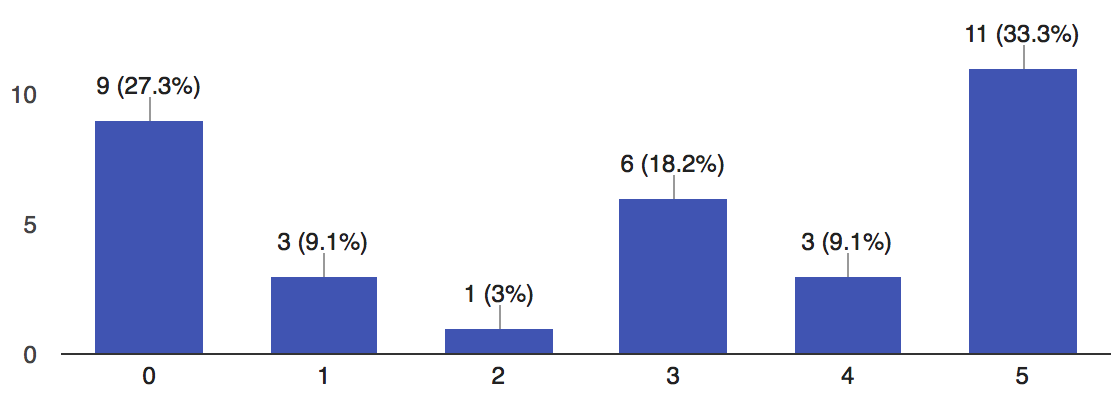
\includegraphics[height=3.2cm]{Banking_with_app}
    \caption{User confidence - logging into bank account via application}
    \label{fig:BankAppConfidence}
\end{figure}

In the case of banking, despite the same number of people who had responded that they did not login to their bank on their device be it via the bank's app or via the mobile web browser, there was a clear shift with our respondents who logged in to their bank on their device, where they were more confident of logging into their bank when using a bank's mobile application instead of the mobile webpage of a bank, accessed on a smartphone's web browser. 42.4\% of our respondents indicated they were confident or very confident with logging in using the bank's app, with 33.3\% out of that 42.4\% going for the very confident option. On the contrary, only 28.2\% of respondents were confident or very confident about logging in via the bank's mobile site. Unfortunately in our study, only a mere 18.2\% of our respondents used a finance management app on their device, and this 18.2\% was almost equally distributed across every confidence option the respondents could choose from - this lack of users of these apps could be down to many users still not adopting such apps (as these apps are generally quite new in the market), or they do not feel confident with them that they do not even use it in the first place.

Shopping with the use of apps too is not widely used in our study group, and we can see near similar results as per the results we obtained from the confidence of users using apps that can charge them money. The number of people who do not conduct this activity is about the same, at 42.4\% instead of nearly 40\% in the case of apps that can charge users for usage, though there were slightly more people who indicated they were at least confident or very confident when conducting such activities. We had 27.3\% of our respondents choosing the confident or very confident option, which is a 3.1\% increase over the proportion of our user base who chose either of these options in the case of using apps that can charge them money.

Our users indicated that they were clearly very confident with accessing work email on their devices, with a clear two-thirds of respondents choosing the very confident option. Aside from the 9.1\% of users who did not use this service, just 12.1\% of respondents did not choose the confident or very confident option - and out of this, not a single person choose the very unconfident option. In the case of working on documents like word processing documents, while a significant chunk of our users (36.4\% of our respondents) did not work on documents on their device, there was a third of our respondents (33.3\%) who indicated they were confident or very confident of working on documents on their device - with nearly double the number of people choosing the very confident option over the confident option. The lack in the number of people who worked on documents is likely due to other factors like file format support by devices, device size and other non privacy and security reasons, as opposed to lack of confidence in their security and privacy being maintained when working on documents on their device.

In the case of giving one's Social Security Number/Social Identity Number (SSN/SIN), a large proportion of our users (72.7\% of users) indicated that they do not do it over an app, or even with the web browser of their smartphone. It was clear in both cases, most of the users who responded that they gave their (SSN/SIN) expressed they were unconfident or very unconfident of their privacy and security when doing this, with more users feeling this way when using an app (24.2\% of users), compared to using the web browser on their smartphone (18.2\% of users in this case chose either one of these options). Not a single user indicated they were very confident, and while 6.1\% of users said they were confident over the web browser,  only 3\% were confident when using an app. The trend that users seemed slightly more confident through the web browser was indeed odd, considering in the case of logging into a bank, our users preferred the app over the use of the web browser.

Health tracking had a reasonable take up rate, with only 45.5\% of our respondents not using this feature. It seemed pretty clear that people seemed confident using this feature, noted by 33.2\% out of the 54.5\% who used this feature indicating that they were confident or very confident of their privacy and security when using this feature. Two thirds of our respondents had indicated that they had used photo sharing features like My Photo Stream/iCloud Photo Sharing (on iOS) or Google Photos (iOS and Android). These apps are designed to automatically (in most cases) upload photos captured on a user's device onto the server of the photo sharing service provider, allowing a user to easily share a photo to others. Our respondents who used it shows that they were pretty neutral in terms of their confidence that their privacy and security was maintained while using such services. 21.2\% of respondents went for the neutral option, while 24.3\% chose either the confident or very confident option, and 21.2\% of users chose either the unconfident or very unconfident option. 

There was a very low take up rate of mobile payment services like Apple Pay and Android Pay, with only 30.3\% of users using this feature. However, it was interesting to note that amongst those who used it, there was almost double the number of people who used this service indicated that they were either confident or very confident that this service ensures their security and privacy is preserved. This is an encouraging trend but we cannot fully conclude this is indeed the current state of the market of mobile payment options, just because many of the respondents did not even use this feature in the first place. One thing to note is that not all banks support this feature and due to that, it would depend on the type of banking services the users use in daily life in order for them to use such mobile payment services. Plus, it could also be due to lack of awareness, as not banks even supported this feature when it was first introduced. Users however seemed quite confident of storing boarding passes and tickets on their devices. 40.6\% out of the 75\% of users who do this indicated they were confident or very confident of their privacy and security when they stored boarding passes and tickets on their device, which was encouraging to see, as it shows that people are comfortable with using their device as a digital wallet.

\begin{figure}[h]
    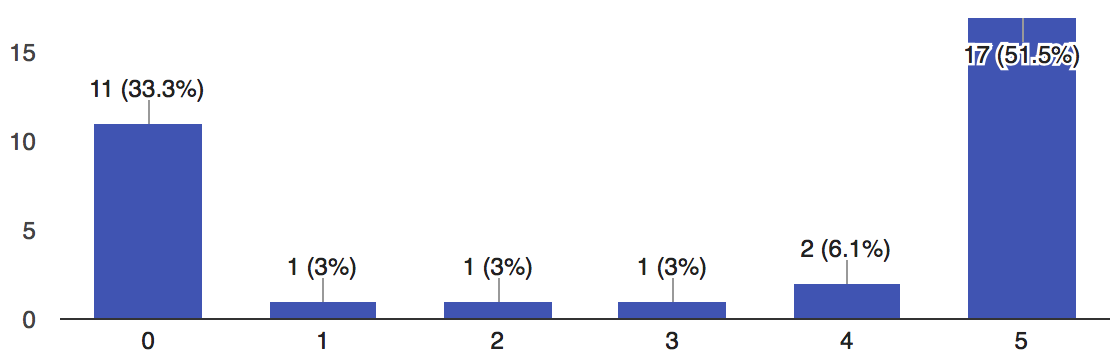
\includegraphics[height=2.95cm]{fingerprint}
    \caption{User confidence with using fingerprint authentication. Option 0 for users who do not use it}
    \label{fig:fingerprint}
\end{figure}

Fingerprint usage to unlock a device too had a high confidence level, out of the 66.7\% of our users who used the feature, 51.5\% chose the very confident option, which again was very encouraging. Only 9\% of all respondents had chosen anything less than the confident option in our questionnaire. Most users however did not use the face unlock feature as for one, it was only available on Android, and even then, it is likely mainly due to the lack of reliability of this feature, especially in poor lighting conditions \cite{lemonnier_2015}. Those who used it, however clearly indicated that they felt very unconfident of their privacy and security, judging by all 12.2\% of respondents who used it ranking it as unconfident or very unconfident. There was an equal number of people for both those ranks. Using a smartphone as a controller for a smart home had slightly better results, again a large proportion of users (78.8\% of our respondents) did not use this feature, but for those who did, 9.1\% ranked it as confident or very confident of their privacy and security when using this, and the same proportion of users ranked it as unconfident or very unconfident. There was 3\% of our population who selected the neutral/average confidence option, which makes it not a clear cut lack of confidence, but rather a case of where we would need more users to try out and use this feature before we can draw solid conclusions - though early signs indicate that it is somewhat well received from the standpoint that the user's privacy and security is not compromised and is maintained while using the smart home controlling features on a smartphone.

\subsection{5.7 Overall User Confidence}

We now present our results from one of the most important parts of our survey. We asked our users, if they felt that they were more concerned about their privacy and security on smartphones compared to their computers. 

\begin{itemize}
\item Security perceptions on smartphones compared to computers

\begin{figure}[h]
    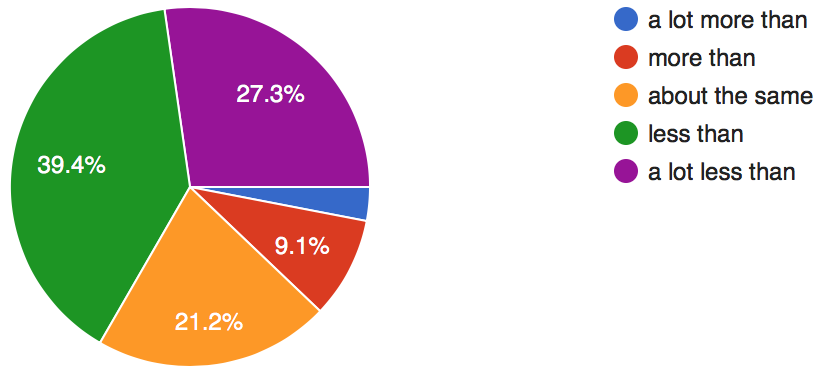
\includegraphics[height=3cm]{securityConfidence}
    \caption{Response for "do you worry about security on the phone \_\_\_\_\_\_  on the laptop"}
    \label{fig:securityConfidence}
\end{figure}

It was very encouraging to see that two-thirds of our respondents (66.7\% of respondents) indicated that they were less or a lot less concerned about security on their smartphones compared to their computer. In fact, just 12.1\% indicated they were more, or a lot more concerned about their security on their smartphone compared to their computer - while the remaining 21.2\% indicated that they had the same level of concern over their security across both devices. This large number of our participants worrying less about their security on their smartphone indicates significant progress over the last couple of years.

We had asked our respondents to explain why they felt a particular way, and it was noted that most of our respondents attributed their lesser concern due to them only installing applications from app stores which are trusted, and ideally have been screened and vetted by the app store provider. This made sense considering all of our users indicated earlier that they only got their apps from their respective app stores. They also felt more secure on their smartphones due to the rather closed nature of smartphones (especially to the normal user) compared to computers, as well as them storing less information on their smartphones. They felt that the closed nature, especially on iOS, helped a lot in ensuring the security of the device.

\item Privacy perceptions on smartphones compared to computers
\begin{figure}[h]
    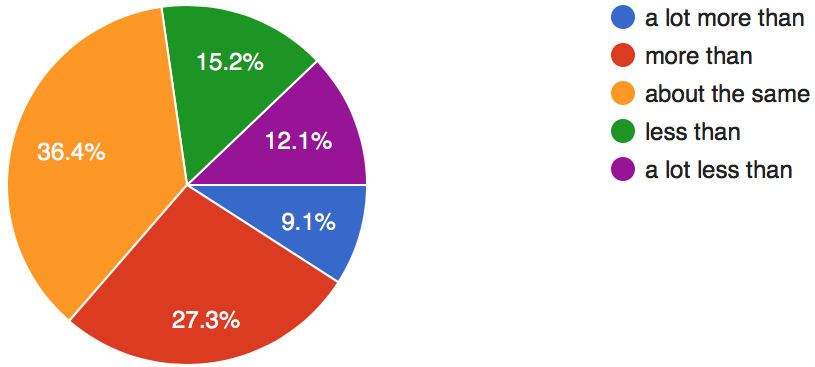
\includegraphics[height=3cm]{privacyConfidence}
    \caption{Response for "do you worry about privacy on the phone \_\_\_\_\_\_  on the laptop"}
    \label{fig:privacyConfidence}
\end{figure}

The positive trend identified in the case of security perceptions does not translate the same way for privacy perceptions, however. 36.4\% of our respondents indicated that they had the same level of concern over their privacy on their smartphone as per their computer. This was larger than the number of people who indicated they worry less, or a lot less about their privacy on their smartphone compared to their computer, as only 27.3\% of our respondents chose either one of those two options. For comparison, this is less than half of the number of people who indicated that they were less or a lot less concerned about their security on their smartphone compared to their computer. In fact, 36.3\% of our respondents indicated they were more, or a lot more, concerned about their privacy on their smartphone compared to their computer - what is interesting is this is nearly the same proportion of our respondents who indicated they had the same level of concern across both their smartphone and computer.

Unlike in the case of security, our further queries with our respondents indicated the reason why our respondents felt this way was quite divided. We received a number of reasons, and among the ones that caught our analysis were that our users were concerned over the fact that that they had their smartphones on them always, and this would allow a lot of data to be collected using the location tracking and sensors built into the device. They also felt not as in control of their privacy on their smartphone unlike on their computers (mainly due to the closed nature of smartphones). Some also mentioned that data is data regardless of where it is, and hence, it is still sensitive while others were concerned due to the fact that smartphones could be easily lost - but at the same time, computers tend to have more data. The amount of data had a play here, as many indicated that they generally had less stored data on their smartphones compared to their computers.

\end{itemize}


We also asked our users if they had any other concerns, aside the ones that have been presented so far, before moving to the next section. Most of our users indicated they were mostly concerned over physical device loss and data leaks or violations, especially if the device was lost. Battery life and open or insecure networks were also other concerns that commonly were mentioned by our users, though not as common as the first two concerns mentioned. There were a few who were also concerned over data violations of the data stores of off site or cloud based backup services they use for their smartphones as well, as well as developers having too much access to information and complicated terms and conditions that they do not end up reading which allows these developers to have this access to their information on their device.
\subsection{5.8 Concerns on Potential Issues with Smartphones}

The idea of this section was to get our respondents to rank the level of concern for a number of potential issues to identify the issues that are important to our users. They were given a 5 point scale, where 1 represented that they were not at all concerned, while 5 was strongly/very concerned.

Based on the data we obtained from our study, we saw that a large proportion of our users indicated that they were at least concerned (or very concerned) about physical phone loss (misplacement or theft) or physical damage of the device, with 75.8\% and 63.6\% of our respondents choosing the concerned or very concerned option for these two issues. Interestingly, for data loss and lack of backups, while 48.5\% of our users were concerned, or very concerned about this, a surprising 42.5\% (near equal) proportion of our users were somewhat unconcerned or not at all concerned over this issue. This may be due to our users feeling like they have less information on their phones compared to their computers, as indicated in the previous section.

A pretty substantial number of our users were at least somewhat concerned, or concerned over reception or signal strength - considering only a third of our users indicated they were somewhat unconcerned or even not at all concerned about this. This was surprising considering that mobile networks have improved significantly over the last couple of years. We also had a large proportion of our users indicating they were concerned (or very concerned) about battery life - which is not surprising considering the current crop of powerful smartphones with large screens that are not able to exhibit the same battery life as per regular mobile phones.

Application trust was a question that yielded interesting results. The concerned option was the most chosen option, with 39.4\% of our respondents choosing this, followed by the somewhat concerned option, which was chosen by 27.3\% of our users. Only 12.1\% of our users had chosen the very concerned option, which was interesting. This leads us to believe while people are concerned about application trust, they are not as concerned as say, physical device loss. We identified that user interface concerns (i.e. unclear user interfaces that do not clearly communicate information, or complicated interfaces that could lead to accidental touches) are relatively strong among our respondents. Only 21.2\% of our respondents had ranked this as either somewhat unconcerned, or not at all concerned. This leads to the remaining being quite concerned - and this is reflected by the 57.6\% of our respondents who indicated that they were at least concerned or very concerned about this issue. This is something that app developers will have to pay more attention to, as if users do not feel confident with using a particular app because it does not clearly communicate information (i.e. an app that involves money that does not indicate the secure connection status, for example), users are less likely to continue using such an application.

We asked our respondents if they had any new concerns that were not addressed in our survey, but there were none that has not been addressed in the survey or the previous sections of this study.

\subsection{5.9 User Feedback on Measures that have been Recommended by Chin et al.}


We finally presented the measures that were recommended by Chin et al. in the original paper, to get our user's feedback on whether they felt that the measures presented were implemented and if they were useful or otherwise. We decided against mentioning that the measures presented in the survey were from Chin et al. for the purpose of getting neutral results and preventing any bias (i.e. the possibility that some respondents knowing the authors of the original paper, hence presenting a biased opinion to us).

In the case of measures to improve user awareness and user education, it was clear that our respondents felt that this measure was not implemented, with over two-thirds of our respondents indicating that they felt this way. Even those who felt otherwise indicated that the effectiveness of this measure has not been very successful. The same sentiment also applied in the case of security indicators in app stores. Many of our users mentioned that they do not think that this measure would be that effective anyway, as they expect the pre-screening done before an app is released for sale on major app stores. This is true, as both Apple and Google have implemented measures to screen apps that are being submitted to their respective app stores for malware and security vulnerabilities \cite{apple} \cite{krill_2012}. Users who agreed that this measure has been implemented mentioned that they have only seen it in third party app stores, and not in the Google or Apple app store. Even then, they did not find these indicators very clear as in many cases, our users said that the indicators were hidden away from direct view.

We had a slightly greater number of respondents who agreed that better user interfaces (UIs) have been implemented to make sensitive apps clearer to users, compared to the number of respondents who disagreed with this. Many of our users who agreed that this measure has been implemented mentioned that it was effective to make the app "feel" more secure, although it does not really make an application inherently more secure. Better interfaces also help to guide the user to avoid mistakes and allow them to clearly understand what is going on. However, our users also mentioned while better user interfaces were there, not all sensitive apps had this, and there is still room for improvement.

In the case of better backup options and better remote locking services, a very significant proportion of our users agreed that these measures have been implemented. While we had a number of users who declined to comment (less than 10 for the backup service and less than 5 for the remote locking service), almost all of the remaining users indicated that they agreed that both of these services have been implemented. Generally our users indicated that the better backup solutions have been effective, but there is room for improvement to make these services less confusing for users to operate. In the case of remote locking services, our users mentioned that this service is effective but has room for improvement to make it easier to use and understand. Users also mentioned that battery consumption by this service could be better optimized in some cases, and that they felt the Android version was not as comprehensive as the iOS version. There is also the lack of assurance in terms protection from the possibility of the device to be compromised via open vulnerabilities in the remote locking services. This is something that is entirely possible, and has plagued the iOS version of remote device tracking and locking, Find My iPhone, as demonstrated earlier this year \cite{vigneswaren_2016}.

\section{6. Comparing with Chin et al.'s result}

In terms of the types of apps, we noticed that messaging and social apps are now the main category of apps installed on user's devices, while entertainment apps have now become the second most popular category. Prior to this, social apps were not too popular, as indicated in the original paper. More people now use the official app stores to get their apps, as noted by all of our respondents who indicated they used the official app stores of their respective platforms, compared to just 85\% of respondents in Chin et al.'s study. What is rather disappointing is that price, popularity and user reviews still remain the top criteria users considered before they obtained an app. The number of people who consider the permissions requested by apps were not too high still, similar to Chin et al.'s study, and the same applies for the number of people who considered the end user license agreement and privacy policy. It was also interesting to note that more people were willing to try unknown brands now, and they generally still heard about apps first from the featured section of the app store, and through the word of mouth (especially from family or friends).

We expected a large proportion of our users to take advantage of the new services like remote device tracking and automated backup services, but interestingly nearly two-thirds of them do not use device tracking services and approximately half of them do not use automatic backup services. However we noted that only one user had an anti-virus app installed.

In terms of user confidence, we still noted a very low level of confidence among our users when dealing with entering their SSN or SIN on their smartphone in general. Significantly more people were confident with having their health data on their smartphone now (through health tracking applications, for example), compared to the earlier study. The same sentiment also applies to banking on their smartphones (especially through the bank's mobile application). While slightly less than 60\% of people shop on their smartphones, the ones who do expressed their confidence while doing so now. Navigation applications that used the user's current location had a very high level of confidence as per the original paper, though it appeared that users seemed less confident with social applications that used their current location in our study. We noted a similar level of confidence for accessing work emails on a smartphone, when comparing Chin et al.'s study with ours.

In terms of the new technologies, our users showed that they were very confident in general with using fingerprint scanners, with a reasonably high take up rate since not all smartphones have this. Face unlock, however, did not have the same level of take up, very few people used this and those who expressed their lack of confidence of their privacy and security when doing so. A large proportion of our users used their smartphones to store passes and tickets, and seemed confident in doing so. The same confidence applied to the use of mobile payment services like Apple Pay and Android Pay, though the take up rate was quite low. We could not conclude the level of confidence of using their smartphones to control smart homes, due to the very low take up rate of this feature.

On a whole, we can say our study has indicated an improvement in terms of perceived smartphone security as less people indicated they were more concerned about security on their smartphone  (down from approximately 40\% of users in Chin et al.'s study to 12.1\% of users now). Those who were equally concerned about security on both their smartphone and computer were the same as the previous study.  Our users have indicated their increased confidence in terms of security due to the screening of apps on the app stores, and the relatively closed nature of mobile OSes, especially iOS, compared to desktop OSes. There were less people who indicated that they are more concerned about their privacy on their smartphone compared to their computer now, with those who feel that they are equally concerned about their privacy regardless of device remaining the same - however the drop in number of users who are more concerned about their privacy on their smartphone was not as big as compared to the drop in the case of users being more worried about security on their smartphone compared to their computer. The reasons for this remain somewhat similar as before, many users attributed the large number of sensors on their smartphones being causes of their concern, although our users mentioned they have less data on their smartphones compared to their computer. The misconceptions in Chin et al.'s paper was not present in our study.

The other concerns presented by our users seemed somewhat similar with what Chin et al. presented, with physical device loss/damage being the main concern, as well as data loss and lack of backup. App trust was something our users were concerned too, but not as highly ranked as physical device loss/damage. Data violations of cloud based backup services (at the data store end) was a new concern, however, and battery life is still a valid concern among our users. Our users generally agreed that the automatic backup and remote device tracking/locking services were generally effective, though they mentioned that there needs to be improvement in terms of raising user awareness and the introduction of security indicators in app stores.

\section{7. Limitation}
Chen's study could have suffered from a \textit{pleasing bias}, where participants tend to say "No" when facing a question in the form of "Would you be willing to do activity X?" in the security context. In order to reduce the risk of bias in our study, we changed the format of the questions into "How confident are you with performing activity X on a scale if 1-5?". Although participants might still answer to this question with a privacy-conscious attitude, we believe results are still more accurate than a "yes" or "no" question.

In terms of our study, we did not separate our users by age and occupation, due to most of our users coming from the same age group and a large proportion of them from the same job field, especially due to our small sample. This may have not allowed us to identify some biases. The use of \textit{Google Forms} had some limitations as we could not really tailor some of the later questions based on the responses provided by our users to earlier questions in the survey.

\section{8. Conclusion}

Our study reveals that today, users feel more confident about their privacy and security on their smartphones, compared to the original study. App selection criteria still remains similar, the EULA, privacy policy and permissions requested by apps still are not the criteria most of our users considered when getting apps. Our users indicated they are now more confident especially with banking and having their health data on their devices, but not with some personal information like their SSN/SIN. Many of the other concerns presented in the original study still apply today as well, especially due to the lukewarm take up rate of automated backup services and device tracking solutions. Our users have indicated some new features, like some (but not all) biometric based authentication systems are well received and have a high user confidence, though some features like mobile payment systems still do not have sufficient take up rates but early signs are encouraging.


%
% References
%
{\footnotesize \bibliographystyle{acm}
\bibliography{reference}}

\appendix

\section{A. Demographics}
\begin{itemize}
\item What is your gender?
\item What is your age?
\item What is your current occupation?
\end{itemize}
\section{B. Mobile Usage}
\begin{itemize}
\item Which smartphone platforms have you used in the past?
\item What platform is your current smartphone based on? If you have more than one phone, answer based on your primary phone that you use most.
\item How much experience do you have with a smartphone?
\item How many people regularly (at least once a week) use this phone?
\item Do you share your phone with any family members / co-workers ?
\item On a scale of 1 (Never) to 5 (Always), please answer the following question: I am likely to try mobile applications made by companies or brands that I am not familiar with
\item What types of applications do you tend to install on your smartphone? 
\item Where do you usually look for applications to install on your smartphone?
\item If there is an “update” available for your Android/iPhone (system update, not individual applications), what do you do?
\item How many applications have you installed yourself (without assistance) on your phone?
\item Do you use lost phone tracking services? (Find My iPhone/Android Device Manager/third-party device tracking services)
\item Do you use data backup services on your smartphone (iCloud Backup/Android Auto Backup/third party data backup solutions)?
\item Do you have any anti-virus or security software installed on your phone? 
\end{itemize}
\section{C. Security Application}
Based on the antivirus/security application that is currently installed on your phone answer the following questions:
\begin{itemize}
\item Name of application?
\item Is it paid or free?
\item Where did you download it from? 
\item How did you first hear about this application?
\item What factors did you consider before installing it? [Price, Popularity of the application, Search ranking/sponsored listing, User reviews, Expert reviews online (blogs, magazines, etc.), Salesperson suggestions in a store (like BestBuy), Family/Friends' recommendations, Familiarity with brand,Ease of installation,Screenshots, End User License Agreements and Terms of Services, The application's privacy policy, Permissions requested from the application]
\item How often do you use it? 
\end{itemize}
\section{D. Non-Security Applications}
\begin{itemize}
\item What categories of applications do you have?
\item Where do you generally get your applications from? 
\item How did you first hear about this application?
\item What factors did you consider before installing it? [Price, Popularity of the application, Search ranking/sponsored listing, User reviews, Expert reviews online (blogs, magazines, etc.), Salesperson suggestions in a store (like BestBuy), Family/Friends' recommendations, Familiarity with brand,Ease of installation,Screenshots, End User License Agreements and Terms of Services, The application's privacy policy, Permissions requested from the application]
\end{itemize}
\section{E. Installation Factors}
Rank the following factors based on one of the available ranks in the dropdown menu [Always Consider,Sometimes Consider,Rarely Consider,Never Consider]:
\begin{itemize}
\item Price
\item Popularity of the application
\item Search ranking/sponsored listing
\item User reviews
\item Expert reviews online (blogs, magazines, etc.)
\item Salesperson suggestions in a store (like BestBuy)
\item Family/Friends' recommendations
\item Familiarity with brand
\item Ease of installation
\item Screenshots
\item End User License Agreements and Terms of Services
\item The application's privacy policy
\item Permissions
\end{itemize}
\section{F. User Confidence Level}
On the scale of 1-5 answer these questions with regard to your confidence level (5 very high and 1 being very low)
\begin{itemize}
\item Using a navigation application on your phone that is location aware? (E.g., Google Maps, Uber)
\item Using a social media application that is location aware? (eg Foursquare, Yelp, Instagram)
\item Usings an application on your phone that can charge you money? (For example, Skype will charge your credit card if you use up your minutes. Some massive player games. Renewal of anti-virus.)
\item Logging into your bank account on your phone using the website?
\item Logging into your bank account on your phone using the app?
\item Using a finance management application on your phone? (E.g., Quicken, Mint)
\item Making a purchase on a shopping site on your phone (via app)?
\item Accessing work-related email on your phone via app?
\item Working on documents (word processing/spreadsheets) on your phone?
\item Giving your Social Security Number/Social Insurance Number  to an application on your phone? (E.g., Tax software, credit check)
\item Giving your Social Security Number/Social Insurance Number  to a website on your phone? (E.g., Tax software, credit check)
\item Using an application to manage your track your health on your phone?
\item Have you used an application to share photos on your phone? (E.g., Google Photos, Apple My Photo Stream/iCloud Photo Sharing)
\item Using mobile payment services like Apple Pay or Android Pay?
\item Store tickets or passes (like boarding passes) on your device?
\item Using Fingerprint scan to access your phone? (iphone)
\item Using Face recognition feature to access your phone? (Android)
\item Control your home with your mobile device (smart lighting - Phillips Hue -  or thermostats - Nest)
\item Do you worry about security (e.g., malicious programs) on the phone [a lot more than | more than | about the same | less than | a lot less than] security on the laptop? Please explain.
\item Do you worry about privacy (e.g., leaking sensitive data) on the phone [a lot more than | more than | about the same | less than | a lot less than] privacy on the laptop? Please explain.
\item In general, what are your primary concerns about your phone?
\end{itemize}
\section{G. User Concerns}
On a scale of 1 (not at all) to 5 (strongly) express how concerned you are about the following situations:
\begin{itemize}
\item Physical phone loss (i.e. via misplacement or theft)
\item Physical damage of device
\item Data loss and lack of backup
\item Reception/signal strength
\item Battery life
\item Application trust
\item User Interface concerns (accidental taps to purchase something)
\item Any new concerns?
\end{itemize}
\section{H. Recommended Measures }
Do you think the following measures have been implemented? if so, how the particular measure helped to improve privacy and security on smartphones?
\begin{itemize}
\item User Awareness/Education: Educating users about the various technologies in place to improve user privacy and security when using a smartphone can help to clear misconceptions.
\item Security indicators for a particular application in app stores: Security indicators would allow users to help judge the "trustworthiness" of an application before they get it from the app store.
\item Better user interfaces for sensitive applications (i.e. banking and taxation applications, applications that perform high value transactions like flight booking applications):Better interfaces can help to increase participants' comfort-level when making critical transactions on their smartphone.
\item Better device backup options (automated or otherwise): Users of mobile devices are concerned of accidental damage, data loss or physical device loss, hence backup solutions can potentially help mitigate these concerns.
\item Better remote device locking services (to secure a device when lost):Ideally remote device locking services would allow users to remotely lock or wipe their devices if they get lost.

\end{itemize}
 \end{document}